
\section{Desarrollo}

Después de haber realizado el análisis inicial de el alcance del proyecto y las necesidades de los usuarios, se comenzó con el desarrollo del proyecto. Este desarrollo se hizo en tres partes. Primero, el desarrollo de un módulo de monitoreo de las estaciones meteorológicas por medio de drivers,  después un API como intermediaria entre la información almacenada en la base de datos y una interfaz gráfica para el monitoreo eficaz.

\subsection{De la base de datos}

Debido a que se seleccionó un sistema basado en un ORM para el manejo de la base de datos, esta tiene que modelarse en el sistema en forma de código para ser reconocida, de la misma forma, la creación de la estructura de la base de datos en el motor se hará por medio de migraciones creadas con el sistema de creación de base de datos, para facilitar su mantenimiento e interoperabilidad en diferentes sistemas y facilitar las integraciones con otros sistemas existentes de información.

Los archivos resultantes de estas migraciones fueron tal como se muestran en el Listado \ref{lst:database-migrations-files}, las cuales se pueden encontrar en la ruta \texttt{/app/database/migrations} del proyecto, tal como es especificado en las guías de desarrollo de MasoniteORM.

\begin{listing}
\begin{minted}{bash}
2021_08_03_052340_stations.py
2021_10_14_162126_station_additional.py
2021_11_13_020934_event_solutions.py            2022_04_03_003436_add_timestamps.py
2021_08_16_000028_station_events.py
2021_10_29_035514_stations.py
2022_03_25_013638_normalize_events_comments.py
2022_04_20_222630_events_fix.py
\end{minted}
\caption{Archivos de migración en el proyecto.}
\label{lst:database-migrations-files}
\end{listing}

Si bien los modelos creados para la ejecución de este proyecto siguen los estándares de modelado de base de datos especificados en MasoniteORM, tal que al modelar la base de datos es posible obtener el mismo código que el implementado, una modificación importante al modelado de los datos es el uso de un mutador para traducir las direcciones IP a enteros y viceversa, como se muestra en el Listado \ref{lst:model-station-mutator}. Este mutador es accesado con un nombre alternativo al nombre del campo en el modelo, debido a que por limitaciones del sistema no es posible utilizar mutadores y accesores con el mismo nombre del campo objetivo.

\begin{listing}
\begin{minted}{python}
import ipaddress
[...]
class Station(Model, UUIDPrimaryKeyMixin, SoftDeletesMixin):
[...]
def get_ip_address_attribute(self):
   return str(ipaddress.ip_address(self.ip))

def set_ip_attribute(self, attribute):
   try:
      ip = ipaddress.ip_address(attribute)
   except ValueError:
      raise ValueError("Invalid IP Address %s" % attribute)

   return int(ipaddress.ip_address(attribute))
\end{minted}
\caption{Definición de accesor y mutador para modelo de estaciones}
\label{lst:model-station-mutator}
\end{listing}

\subsection{Del módulo de monitoreo de las estaciones}

Para realizar la conexión a las estaciones meteorológicas, se decidió dividir el proyecto en dos componentes principales, un módulo de generación de reportes y un sistema de controladores que contuvieran el código de conexión y restauración de reportes de las estaciones.

Tomando como referencia el proyecto de \textit{Monitoring Plugins} \cite{monitoring_plugins}, el cual es compatible con diversos proyectos especializados en monitoreo de sistemas de alta resilencia, tales como \textit{Nagios} y \textit{Icinga}, se decidió crear un proyecto basado en drivers que pudieran ser extendibles. Cada uno de estos drivers, puede cargar una cantidad \textit{n} de módulos o servicios, que contienen la información necesaria para obtener el estado de la estación meteorológica y saber si están funcionando de forma correcta o no.

Con el objetivo de crear un sistema que fuera posible integrar en diferentes ambientes y no requiriera de previa instalación de componentes extra en el dispositivo objetivo, se decidió que la información con la que se revisaría el estado de las estaciones es por medio de un comando que se ejecutaría en una estación remota, o de forma local dado el caso, y se comparara la respuesta obtenida con el resultado de la operación. En caso de que la respuesta de esta operación sea diferente a la respuesta esperada, se buscará en un arreglo de casos conocidos, que pueden ser solucionados con la ejecución de un comando.

La estructura del servicio es un objeto con la forma que se puede apreciar en el Listado \ref{lst:service-example}, donde el arreglo de casos conocidos tiene el nombre de \textit{actions}, y es anidable, lo que permite listar una serie de comandos que pueden ayudar a la solución de problemas con una produndidad \textit{n}.

\begin{listing}
\begin{minted}[%
   breaklines
]{python3}
service = {
   "command": "", # Comando a ejecutar
   "stdout": "", # Salida esperada
   "stderr": "", # Error esperado
   "actions": {
      "read_write_enabled": {
         "response_stdout": "", # Si la respuesta del comando previo es esta
         "response_stderr": "", # Si el error del comando previo es este

         "description": "", # Descripción para el usuario del error
         "solution": "", # Solución propuesta, si existe, para el usuario

         "command": "", # Comando a ejecutar
         "stdout": "", # Salida esperada
         "stderr": "", # Error esperado
         "actions": {
            # ...
         }
      }
   }
}
\end{minted}
\caption{Ejemplo de estructura de un servicio}
\label{lst:service-example}
\end{listing}

Para el desarrollo de la estructura del \textit{driver} de monitoreo de las estaciones meteorológicas, se optó por crear un sistema orientado a la extensión de un componente base que fungiera como sistema principal de ejecución, verificación de credenciales y ejecución de comandos en el sistema objetivo. La estructura de los drivers para el acceso a la información quedó tal como es posible observar en la Figura \ref{fig:diagrama_clase_drivers}.

\begin{figure}[!ht]
	\centering
	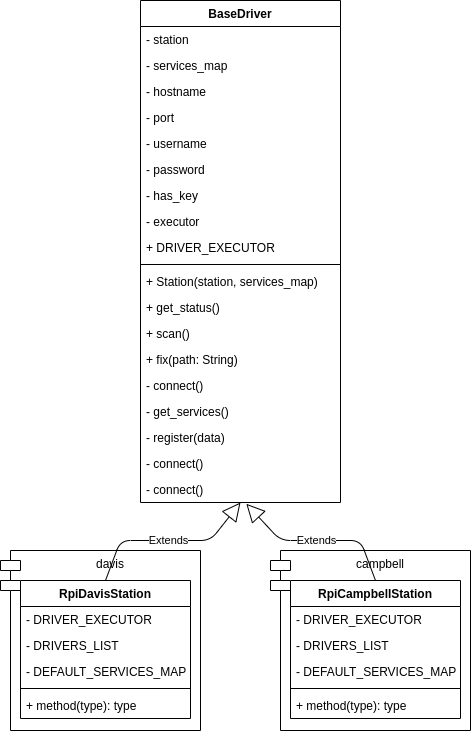
\includegraphics[width=0.2\linewidth]{images/diagrams/classes/drivers.drawio.png}
	\caption{Diagrama de clase de drivers}
	\label{fig:diagrama_clase_drivers}
\end{figure}

Para los ejecutores, tal como se muestra en el diagrama de clases de la Figura \ref*{fig:diagrama_clase_ejecutores}

\begin{figure}[!ht]
	\centering
	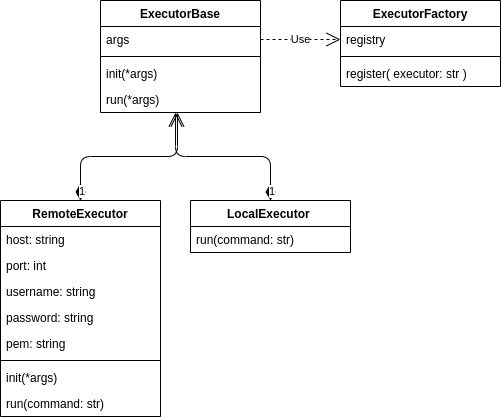
\includegraphics[width=0.6\linewidth]{images/diagrams/classes/executors.drawio.png}
	\caption{Diagrama de clase de ejecutores}
	\label{fig:diagrama_clase_ejecutores}
\end{figure}




\begin{figure}[!ht]
	\centering
	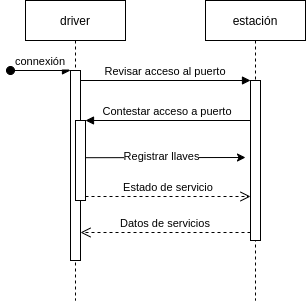
\includegraphics[width=0.5\linewidth]{images/diagrams/classes/registering_execution.drawio.png}
	\caption{Diagrama de clase de drivers}
	\label{fig:diagrama_de_ejecución}
\end{figure}


\subsection{Del módulo de monitoreo de estaciones}

El módulo de monitoreo de estaciones meteorológicas tiene como objetivo el observar la información obtenida por los diversos drivers de conexión a las estaciones meteorológicas y generar reportes conforme sea necesario, la lógica de reporte es tal como se muestra en la figura \ref{fig:logica_de_reporte}.

%! Agregar acciones al diagrama
%! Cambiar por diagrama de secuencia
% Agregar un fin después de generar la alerta
% debe hber un solo inicio y final

\begin{figure}[!ht]
	\centering
	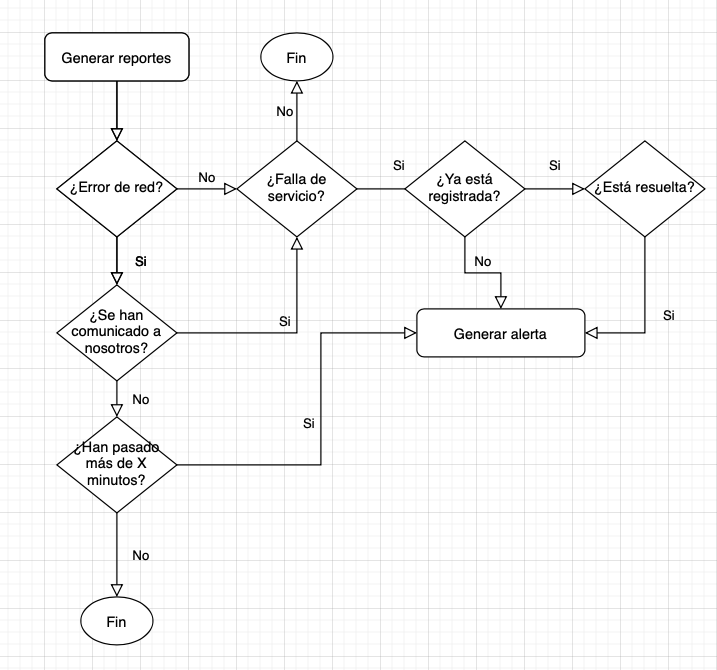
\includegraphics[width=1\linewidth]{images/diagrams/report_logic.png}
	\caption{Lógica de reporte del estado de las estaciones meteorológicas}
	\label{fig:logica_de_reporte}
\end{figure}


\subsection{Del API para el acceso a la información}

\subsection{De la interfaz gráfica del proyecto}

PAra el desarrollo del proyecto, se utilizó tailwind.

\subsection{De la documentación}

Un sistema es tan bueno como su documentación.

\section{Avances}


\section{Módulo de monitoreo}

\subsection*{Requisitos}

\subsection*{Seguridad}

\subsection*{Método de conexion}



\section{Selección de base de datos}

%! Terminar para la próxima

% Casi todas las secciones de desrrollo, van ligadas a una de resultados.

%? Escribir el proceso que realicé. Presentar lo suficiente para darle una idea al lector.

%? Presentar un fragmento de código más relevante. Incluir enlace a repositorio. La funcionalidad se puede expresar en algún tipo de representación gráfica.

%? Evitar párrafos de una sola oración. (Dar MÁS contexto), extranjerismos en itálica.
Con un tiempo de respuesta de $~[N]ms$, el sistema puede soprotar hasta N estaciones concurrentes.

Debido a que la recolección de los datos es por métodología pull y no push, es posible tener las estaciones en una cola que se ejecute hasta por un periodo de 5 minutos (que es un estándar en la recolección de datos de estaciones meteorológicas). Esto implica que la base de datos [X] puede soportar hasta [N x 60 x 5] datos de forma concurrente.

Tomando en cuenta las necesidades actuales del LCCA, y el estimado del tamaño de las redes de alta densidad (que pueden llegar hasta los N nodos como X artículo lo demuestra), no vale la pena el introducir la complejidad extra de un motor de base de datos desconocido y para el que no existen ORM's con soporte completo en el lenguaje de desarrollo. Porque no es un sistema de alta densidad de datos.

Si bien es posible escalar horizontalmente la infraestructura, se busca evitarlo ya que los \textit{diminishing returns} del costo de tener que mantener un sistema de monitoreo no es costeable. Para los casos de sistemas de extremadamente alta densidad, se recomienda el crear varias instancias seccionadas en bases de datos, o escalar la base de con un redis en vez de escalar.

%! Recordar que la información debe ser consultada desde el API, así que no sólo se tienen que tomar en cuenta la cantidad de query's por segundo que se requieren hacer para las inserciones, sino también para la consulta de datos.

%! Si lo que queremos es proveer herramientas para la gestión de calidad de los datos meteorológicos, la información tiene que tener en mente los principios Solidos y transaccionales, al menos en la creación de reportes basados en incidentes.

\subsection{Selección del motor de base de datos}

Para el caso de uso del centro de monitoreo de estaciones meteorológicas de la UACJ, en el que la red actual cuenta con 13 estaciones, no es necesario considerar como cuello de botella el motor de base de datos que se utilizará para el sistema. Esto debido a que, con un tiempo mínimo para la consulta del estado de las estaciones de hasta 5 minutos entre consultas, el sistema podría funcionar incluso con un tiempo promedio de 23 segundos desde la consulta hasta el almacenamiento de la información. Esto, sin tomar en cuenta que es posible paralelizar el proceso de consulta y generación de eventos de las estaciones meteorológicas, por lo que no se considera como algo relevante la selección de un motor de base de datos que cuente con alto rendimiento de lectura y/o escritura de la información.

Debido a que la infraestructura del sistema de las estaciones meteorológicas ya utiliza un motor relacional de base de datos adecuado para el proyecto, MySQL, se pretende utilizarlo para este proyecto, reduciendo la carga de mantenimiento para el equipo de la universidad, además de un sistema familiar que permitirá a los involucrados realizar consultas a la información sin necesidad de aprender nuevas tecnologías.

Para esto, se utilizó la flexibilidad que ofrecen los sistemas modelado de objetos y roles (ORM, por sus siglas en inglés) \cite{Halpin2006}, en la que se permite el crear sistemas agnósticos de un motor de base de datos en específico, y la creación de modelos, esquemas y relaciones de base de datos se dejan al \textit{framework} de modelado de datos. Esto además ofrece soporte para migraciones para realizar actualizaciones de base de datos controladas en caso de requerir extender un sistema existente.

El motor de base de datos seleccionado para el desarrollo local del proyecto fué el conocido como \textit{SQLite}, debido a la flexibilidad que ofrece al ser una base de datos que sólo depende de un archivo para funcionar y que no requiere de instalar paquetes de software extra en la estación que se utiliza para desarrollar y probar el proyecto.
